% this file is called up by thesis.tex
% content in this file will be fed into the main document

\chapter{Technical Approach} \label{ch:chapter3} % top level followed by section, subsection

\ifpdf
    \graphicspath{{3_chapter3/figures/PNG/}{3_chapter3/figures/PDF/}{3_chapter3/figures/}}
\else
    \graphicspath{{3_chapter3/figures/EPS/}{3_chapter3/figures/}}
\fi

% ----------------------- contents from here ------------------------
\section{Study Design}

\gls{TILDA} provides longitudinal data across five waves for community dwelling adults in Ireland. This thesis uses data from five core \gls{TILDA} waves (Waves 1--5). For contextual comparison and benchmarking against international cohorts (see Chapter~\ref{ch:chapter1}) however, it is important to note this is an external resource and not the output of the thesis's primary preprocessing pipeline. The primary analytical work focuses on the full five wave \gls{TILDA} dataset.

\section{Cohort Definition}

All participants who provided data in at least one \gls{TILDA} wave were considered eligible. To maximise the available sample for machine learning, no exclusions were applied on the basis of age, medical conditions, mobility, cognitive status, or health centre attendance.

Participants were removed only when, after the combined manual filtering and automated preprocessing pipeline, they had no remaining usable variables. Filtering therefore occurred primarily at the \emph{variable level}, with features removed for extreme missingness, lack of variation, or non informative structure (see Chapter~\ref{ch:chapter4}). This approach preserves the largest possible sample while ensuring all retained inputs are analytically meaningful.

\subsection{Cohort inclusion criteria}
\begin{itemize}
    \item \textbf{Participant inclusion:} All respondents who contributed data in at least one wave were included in the initial sample.
    \item \textbf{Usable data requirement:} Participants were excluded only when, after manual filtering and preprocessing, no usable variables remained.
    \item \textbf{Longitudinal retention:} Individuals were retained regardless of how many waves they contributed to, enabling initial maximum dataset utilisation.
    \item \textbf{No clinical exclusions:} No participant was removed due to medical diagnoses, cognitive scores, functional limitations, or non attendance at the health centre assessment.
\end{itemize}
This approach prioritises data integrity and sample size for machine learning applications rather than clinical eligibility criteria common in classical epidemiological analyses.

\section{Data Collection}

Data used in this thesis were collected across five waves:
\begin{itemize}
    \item \textbf{Wave 1:} 2009--2011
    \item \textbf{Wave 2:} 2012--2013
    \item \textbf{Wave 3:} 2014--2015
    \item \textbf{Wave 4:} 2016--2018
    \item \textbf{Wave 5:} 2018--2020
\end{itemize}

All \gls{TILDA} data were pseudonymised prior to release. Each participant received a unique identifier (`id') along with household and cluster identifiers (`household', `cluster') to permit longitudinal linkage while preserving anonymity. Each wave included three primary components:
\begin{enumerate}
    \item \textbf{\gls{CAPI}:} Home based, computer assisted personal interviews covering health, socio demographics, and family.
    \item \textbf{\gls{SCQ}:} Paper based self completion questionnaires capturing sensitive information on mental health, lifestyle, and wellbeing.
    \item \textbf{Health Assessment:} Clinical and biomarker measurements conducted in dedicated centers or at home (Wave 1 and Wave 3).
\end{enumerate}

\subsection{Data Overview}
Before processing, raw \gls{TILDA} datasets were manually inspected, and clearly non informative variables (e.g., administrative identifiers, constant columns, high missingness) were removed. Table~\ref{tab:raw_dataset_shape} shows the raw dimensions of each dataset.

\begin{table}[htbp]
\centering
\caption{Dimensions of Raw \gls{TILDA} and Harmonised Datasets (Pre Filtering)}
\label{tab:raw_dataset_shape}
\begin{tabular}{|c|c|c|}
\hline
\textbf{Dataset} & \textbf{Participants (N)} & \textbf{Raw Variables (N)} \\
\hline
Wave 1 & 8501 & 1619 \\
Wave 2 & 7206 & 724 \\
Wave 3 & 6397 & 1029 \\
Wave 4 & 5713 & 990 \\
Wave 5 & 4978 & 983 \\
Harmonised \gls{RAND} & 8501 & 572 \\
\hline
\end{tabular}
\end{table}

\subsection{Variable filtering criteria}
Manual filtering used rules-of-thumb prior to automated cleaning:
\begin{itemize}
    \item \textbf{Missingness:} Drop variables with $>80\%$ missing values.
    \item \textbf{Unique values:} Drop variables with a single value, flag small cardinality variables (2--10 unique values) for retention.
    \item \textbf{Dominant category:} Flag variables with extremely frequent categories (e.g., $>90\%$) for review.
    \item \textbf{Identifiers / administrative fields:} Obvious IDs, version tags, and sampling weights were identified using the \gls{PMF} metadata. Variable names and descriptions were exported from each wave's \gls{PMF} file into CSV files (code provided in Appendix~\ref{app:pmf_code} ) to systematically document and review features prior to filtering. This ensured analytic relevance and traceability.
\end{itemize}

These manual checks produced a reduced variable set, subsequently processed using the automated six scenario cleaning engine (Chapter~\ref{ch:chapter4}).

\subsection{Variable filtering flowchart}
Figure~\ref{fig:variable_filter_criteria} shows the stepwise variable filtering process. This flowchart guided the removal or flagging of variables based on missingness, low variation, dominant categories, or irrelevance. Dimensionality reduction improved interpretability while preserving longitudinal structure for feature engineering and machine learning.

\begin{figure}[htbp]
\centering
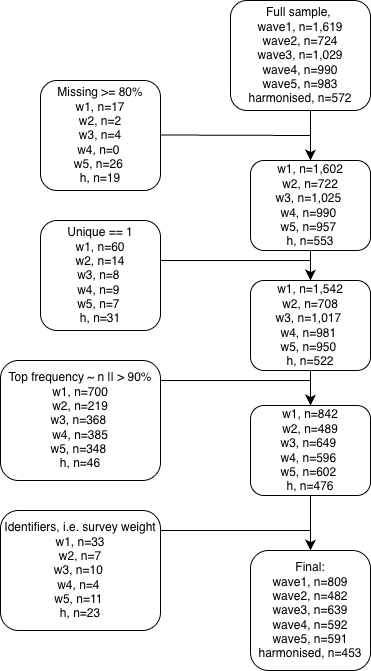
\includegraphics[height=1.25\textwidth]{variable_filter_criteria.png}
\caption{Flowchart of the manual variable filtering criteria. Placeholder counts indicate remaining variables per dataset after each step.}
\label{fig:variable_filter_criteria}
\end{figure}

\section{Thematic Grouping}

After manual filtering, retained variables were organised into six thematic domains aligned with ageing literature and study objectives. The grouping process followed the standard \gls{PMF} naming conventions (Table~\ref{tab:pmf_prefixes}). Specifically, each variable's prefix indicated its data source or domain, which allowed us to systematically assign variables to one of six thematic domains. This ensured that features included in each domain were conceptually coherent and analytically meaningful. 

\subsection{Derived variable prefixes}

To systematically process \gls{TILDA} variables, each variable was assigned a prefix indicating its data source or research domain. Variables collected through the home based \gls{CAPI} follow a two letter module code plus three digit question code format (e.g., \texttt{ph121}). For questions with multiple responses or loops across participants or objects, an underscore and number indicates the specific response or loop iteration (e.g., \texttt{ph201\_05}).

Variables from the self completion questionnaire (\gls{SCQ}) are prefixed with `\gls{SCQ}'. Derived variables, constructed from either \gls{CAPI} or \gls{SCQ} data, use an uppercase code corresponding to the research area (Table~\ref{tab:pmf_prefixes}). These prefixes provide a consistent framework for categorising variables and underpin the subsequent assignment of features into thematic domains for downstream analysis.

\begin{table}[htbp]
\centering
\caption{PMF Derived Variable Prefixes and Research Areas (\cite{tilda2023pmf})}
\label{tab:pmf_prefixes}
\begin{tabular}{|l|l|}
\hline
\textbf{Variable Prefix} & \textbf{Research Area} \\
\hline
ADL & Activities of daily living \\
BEH & Health behaviours \\
BLOODS & Blood sample results \\
BP & Blood pressure \\
COG & Cognitive scales and questions \\
CRT & Choice reaction time \\
DIS & Disability, functional impairment, helpers \\
FR & Frailty, gait, exercise, falls \\
G2G & Gateway to Global Aging Data \\
GRIP & Grip strength \\
IADL & Instrumental activities of daily living \\
INC & Income variables \\
MD & Medication data \\
MH & Mental health scales and questions \\
SCR & Screening tests \\
SES & Socio-economic class variables \\
SOC & Social support and relationships \\
\hline
\end{tabular}
\end{table}

\subsection{Feature groups}

Using the \gls{PMF} prefixes as a guide, variables were systematically mapped to six thematic groups (Table~\ref{tab:feature_groups}). Each thematic group captures a conceptually coherent domain, reflecting physical, cognitive, social, and behavioural aspects of ageing. This categorisation served two key purposes in the thesis: 

1. It structured the data for the automated six scenario cleaning engine (Chapter~\ref{ch:chapter4}), ensuring consistent application of filtering rules and facilitating reproducible preprocessing.

2. It aligned feature selection with the analytic focus of the thesis, enabling machine learning models to leverage variables that are both conceptually meaningful and longitudinally robust across multiple waves.

The six thematic groups integrate information from \gls{CAPI}, \gls{SCQ}, and derived variables, covering socio demographic context, physical health, functional status, lifestyle behaviours, nutrition/metabolic biomarkers, and psychological/cognitive measures. This structured grouping enhances interpretability, ensures comprehensive domain coverage, and provides a foundation for downstream predictive modelling and risk assessment.

\begin{table}[htbp]
\centering
\caption{Thematic grouping of longitudinal features}
\label{tab:feature_groups}
\begin{tabular}{|c|p{4cm}|p{5cm}|p{5cm}|}
\hline
\textbf{ID} & \textbf{Thematic Group} & \textbf{Description} & \textbf{Representative Variables} \\
\hline
1 & Socio Demographic \& Context & Baseline stratification factors & Age, Gender, Education, \gls{INC}, Marital Status, \gls{SOC} \\
2 & Physical Health \& Clinical Baseline & Self reported and clinical indicators & Self Rated Health \gls{SCR}, \gls{BMI}, \gls{BP}, Comorbidity Count \gls{MD} \\
3 & Functional Status \& \gls{FR} & Measures of mobility and physical decline & \gls{FR} Index \gls{FR}, \gls{UGS}, Falls History \textit{SCQFalls}, \gls{IADL} \gls{DIS} \\
4 & Lifestyle \& Behavioural & Modifiable health related behaviours & Smoking, Alcohol Intake \textit{SCQAlco}, \gls{PA} \gls{IPAQ} \\
5 & Nutrition \& Metabolic Biomarkers & Objective nutritional and metabolic markers & Plasma Carotenoids, Lutein, Zeaxanthin, Vitamin D/B12, Cholesterol \\
6 & Psychological \& Cognitive & Mental health and cognitive performance & \gls{CESD}, Loneliness \textit{MHucla}, \gls{COG}, \gls{CRT} \\
\hline
\end{tabular}
\end{table}